\documentclass[prl,twocolumn]{revtex4-1}
\usepackage{graphicx}
\usepackage{amsmath}
\usepackage{hyperref}
\usepackage{booktabs}
\usepackage{xcolor}

\usepackage{siunitx}

\setlength{\tabcolsep}{10pt}

\newenvironment{sistema}%
  {\left\lbrace\begin{array}{@{}l@{}}}%
  {\end{array}\right.}


\usepackage{pgfplots}
\usepgfplotslibrary{external}
\usepgfplotslibrary{groupplots}
\usepgfplotslibrary{units}
\usepgflibrary{decorations.shapes, decorations.fractals}
\usetikzlibrary{positioning, plotmarks, matrix, fit, shapes.geometric}
\tikzexternalize
%\tikzset{external/force remake}
\tikzset{every mark/.append style={scale=0.8}}
\pgfplotsset{every axis/.append style={small}}
\usepackage{pgfplots}
\pgfplotsset{compat=1.9}
\usepgfplotslibrary{groupplots}
\usepgfplotslibrary{external}
\tikzexternalize
\tikzsetexternalprefix{figs/}

\begin{document}
\tikzset{external/force remake=false}
\begin{figure*}
	\centering
	\begin{tikzpicture}[
		pic3d/.style={inner sep=0}, %
		lab/.style={below right, text height=0.8em, text depth=0.2em, font=\Large\bfseries},%
		]%
		\begin{scope}[xshift=0.1\textwidth, yshift=-0.025\textwidth]
			%\fill[blue!10] (0.01\textwidth,0) rectangle (0.2\textwidth, 0.19\textwidth);
			\draw (0, 0.12\textwidth) rectangle (0.01\textwidth,0) %
				(0.2\textwidth, 0.12\textwidth) rectangle (0.21\textwidth,0)%
				(0, 0.13\textwidth) rectangle (0.01\textwidth,0.19\textwidth)%
				(0.2\textwidth, 0.13\textwidth) rectangle (0.21\textwidth,0.19\textwidth)%
				(0, 0.19\textwidth) rectangle (0.21\textwidth, 0.195\textwidth);		
			\filldraw[gray] (0, 0.12\textwidth) rectangle (0.038\textwidth, 0.13\textwidth) 
				(0.042\textwidth, 0.13\textwidth) rectangle (0.098\textwidth, 0.12\textwidth)
				(0.102\textwidth, 0.13\textwidth) rectangle (0.158\textwidth, 0.12\textwidth)
				(0.162\textwidth, 0.13\textwidth) rectangle (0.21\textwidth, 0.12\textwidth);
			\fill[green, semitransparent] (0.1\textwidth, 0.17\textwidth) -- (0.06\textwidth, 0.22\textwidth) -- (0.14\textwidth, 0.22\textwidth) -- cycle;
			\filldraw[lightgray] (0.05\textwidth, 0.22\textwidth) arc[start angle=180,delta angle=180,x radius=0.05\textwidth, y radius=0.01\textwidth] --cycle;
			\begin{scope}[radius=0.008\textwidth, ball color=red!80]
				\shade(0.08\textwidth, 0.175\textwidth) circle;
				\shade(0.11\textwidth, 0.16\textwidth) circle;
				\shade(0.05\textwidth, 0.15\textwidth) circle;
				\shade(0.03\textwidth, 0.18\textwidth) circle;
				\shade(0.14\textwidth, 0.14\textwidth) circle;
				\shade(0.16\textwidth, 0.165\textwidth) circle;
			\end{scope}
			\draw[%
				gray, decoration={coil, segment length=0.0025\textwidth, amplitude=0.0025\textwidth},
				]
				(0.06\textwidth, 0.1745\textwidth)
				decorate{++(-0.0025\textwidth,-0.0025\textwidth) -- ++(0.0045\textwidth,0.0045\textwidth) -- ++(0,-0.0045\textwidth) -- ++(-0.005\textwidth,+0.005\textwidth) }
				(0.17\textwidth, 0.1345\textwidth)
				decorate{++(-0.0025\textwidth,-0.0025\textwidth) -- ++(0.0045\textwidth,0.0045\textwidth) -- ++(0,-0.0045\textwidth) -- ++(-0.005\textwidth,+0.005\textwidth) }
				(0.172\textwidth, 0.14\textwidth)
				decorate{++(-0.0025\textwidth,-0.0025\textwidth) -- ++(0.0045\textwidth,0.0045\textwidth) -- ++(0,-0.0045\textwidth) -- ++(-0.005\textwidth,+0.005\textwidth) }
				(0.145\textwidth, 0.16\textwidth)
				decorate{++(-0.0025\textwidth,-0.0025\textwidth) -- ++(0.0045\textwidth,0.0045\textwidth) -- ++(0,-0.0045\textwidth) -- ++(-0.005\textwidth,+0.005\textwidth) }
				(0.19\textwidth, 0.18\textwidth)
				decorate{++(-0.0025\textwidth,-0.0025\textwidth) -- ++(0.0045\textwidth,0.0045\textwidth) -- ++(0,-0.0045\textwidth) -- ++(-0.005\textwidth,+0.005\textwidth) }
				(0.09\textwidth, 0.14\textwidth)
				decorate{++(-0.0025\textwidth,-0.0025\textwidth) -- ++(0.0045\textwidth,0.0045\textwidth) -- ++(0,-0.0045\textwidth) -- ++(-0.005\textwidth,+0.005\textwidth) }
				(0.03\textwidth, 0.15\textwidth)
				decorate{++(-0.0025\textwidth,-0.0025\textwidth) -- ++(0.0045\textwidth,0.0045\textwidth) -- ++(0,-0.0045\textwidth) -- ++(-0.005\textwidth,+0.005\textwidth) }
				;
			\begin{scope}[blue, every node/.style={circle, inner sep=0.002\textwidth, fill}]
				\draw[decorate,decoration={shape backgrounds,shape=circle,shape size=0.002\textwidth}, fill=blue, step=0.01\textwidth] %
				(0.012\textwidth,0) grid (0.19\textwidth, 0.08\textwidth);
				\draw[decorate,decoration={shape backgrounds,shape=circle,shape size=0.002\textwidth}, fill=blue, step=0.017\textwidth] %
				(0.012\textwidth, 0.08\textwidth) grid (0.195\textwidth, 0.115\textwidth);
				%(0.17\textwidth,  0.0745\textwidth) -- (0.145\textwidth, 0.05\textwidth) -- (0.0514\textwidth, 0.09\textwidth)%
				%(0.03\textwidth, 0.045\textwidth) -- (0.07\textwidth, 0.07\textwidth);
			\end{scope}
			\begin{scope}[blue!20,->, line width=0.005\textwidth]
					\draw (0.16\textwidth, 0.08\textwidth) -- (0.16\textwidth, 0.11\textwidth);
					\draw (0.1\textwidth, 0.08\textwidth) -- (0.1\textwidth, 0.11\textwidth);
					\draw (0.04\textwidth, 0.08\textwidth) -- (0.04\textwidth, 0.11\textwidth);
			\end{scope}
			\node[lab, above right=0, inner sep=0] at (0, 0.195\textwidth) {a};
			\begin{scope}[right, font=\footnotesize]
				\node at (0.21\textwidth,0.21\textwidth) {Objective lens};
				\node at (0.21\textwidth,0.17\textwidth) {Observation cell};
				\node at (0.21\textwidth,0.125\textwidth){Filter};
				\node[above right,blue] at (0.21\textwidth,0.08\textwidth) {Salt diffusion};
				\node[above right] at (0.21\textwidth, 0) {Reservoir};
			\end{scope}
		\end{scope}
		
		
		\begin{semilogyaxis}[%
			at={(0.5\textwidth,0)}, anchor=left of south west,%
			name={phasediag},%
			width=0.425\textwidth, height=0.3\textwidth,%
			xmin=0, xmax=40, xlabel={$\phi$}, x unit={\%},
			ymin=0.08, ymax=3.5, ylabel={$c_p$}, y unit={\si{\gram\per\litre}},%
			ytick={0.1,0.2,0.3,0.4,0.5,0.6,0.7,0.8,0.9,1,2}, yticklabels={0.1,0.2,,,0.5,,,,,1,2},%
			legend pos=outer north east,%
			legend style={font=\footnotesize},%
			only marks,%
			]%
			\addplot[sharp plot, no marks] table [x expr=100*\thisrowno{0}, y index=1] {gasliquid_sg.phd};
			\addplot[sharp plot, no marks, dashed] table [x expr=100*\thisrowno{0}, y index=1] {gasliquid_bg.phd};
			\addplot[sharp plot, no marks, dotted] table [x expr=100*\thisrowno{0}, y index=1] {fluidsolid_f.phd};
			%\addplot+[forget plot] table [x index=1,y index=2] {phase_diag_capillary.csv};
			\addplot table [x index=1,y index=2] {phase_diag_gel.csv};
			\addplot table [x index=1,y index=2] {phase_diag_fluid.csv};
			\addplot table [x index=1,y index=2] {phase_diag_transient.csv};
			\legend{spinodal, binodal, gas-solid, gel, fluid, transient};
			\node[circle, draw, gray] at (axis cs:7.4, 0.98) (155C) {};
			\node[draw, gray] at (axis cs:30, 1) (Cap1) {};
		\end{semilogyaxis}
		\node[lab] at (phasediag.outer north west) {b};
		
		\begin{scope}[pic3d]
			\node[below left=0 of phasediag.outer south east] (threeD_20min) {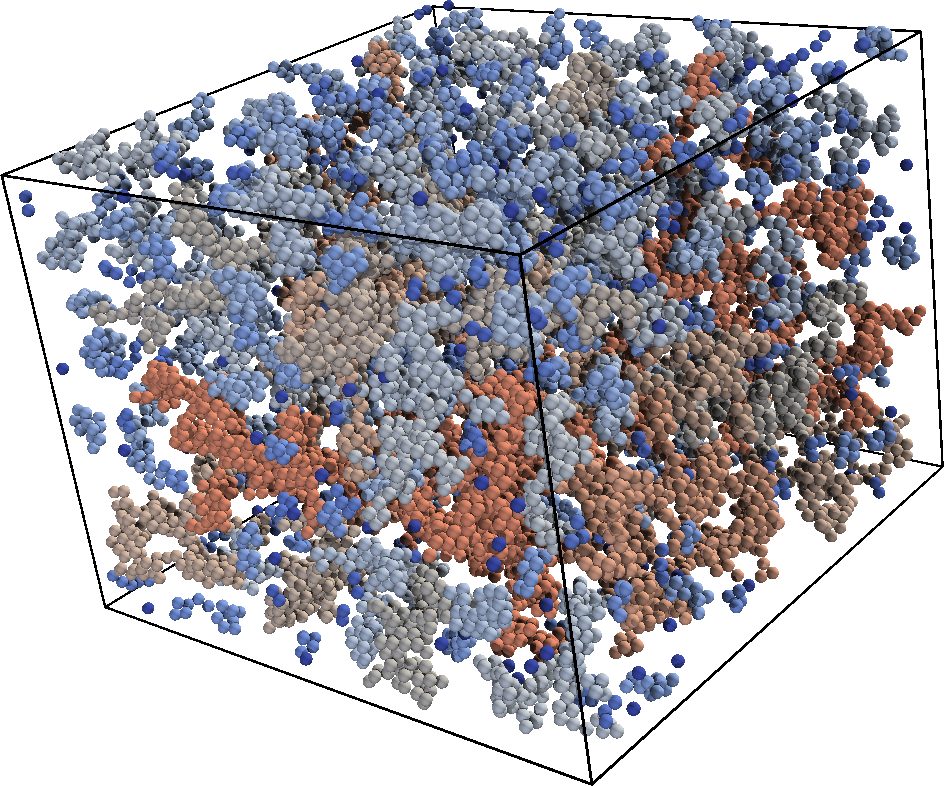
\includegraphics[width=0.3\textwidth]{155C_percolation_1645_p2size_t084.png}};
			\node[left=0.01\textwidth of threeD_20min] (threeD_10min){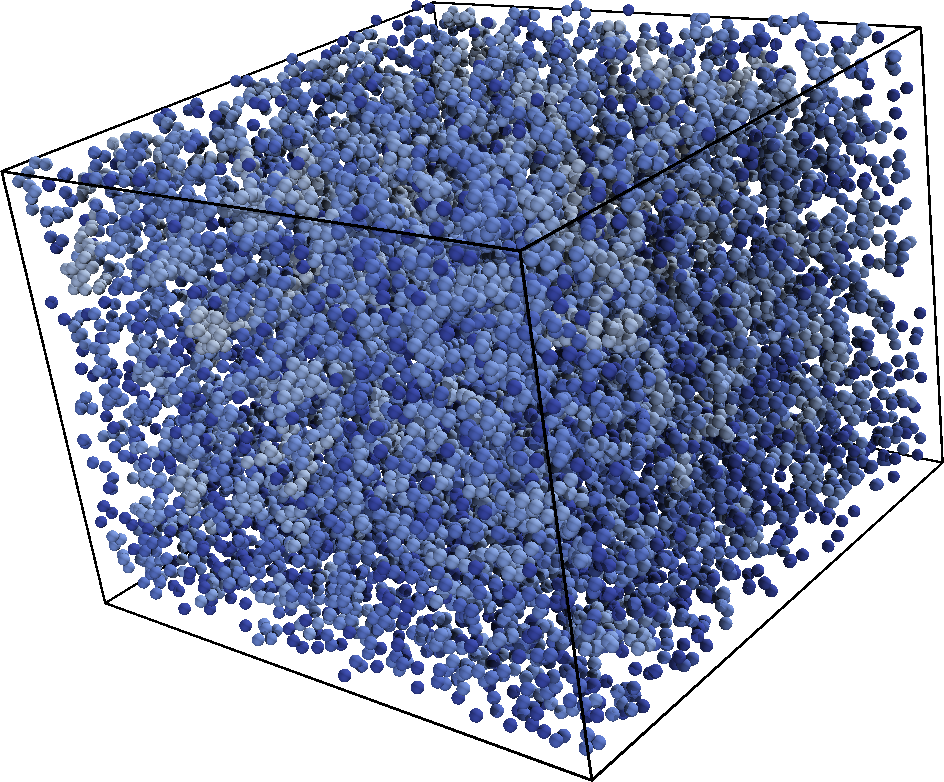
\includegraphics[width=0.3\textwidth]{155C_percolation_1645_p2size_t044.png}};
			\node[left=0.01\textwidth of threeD_10min] (threeD_5min) {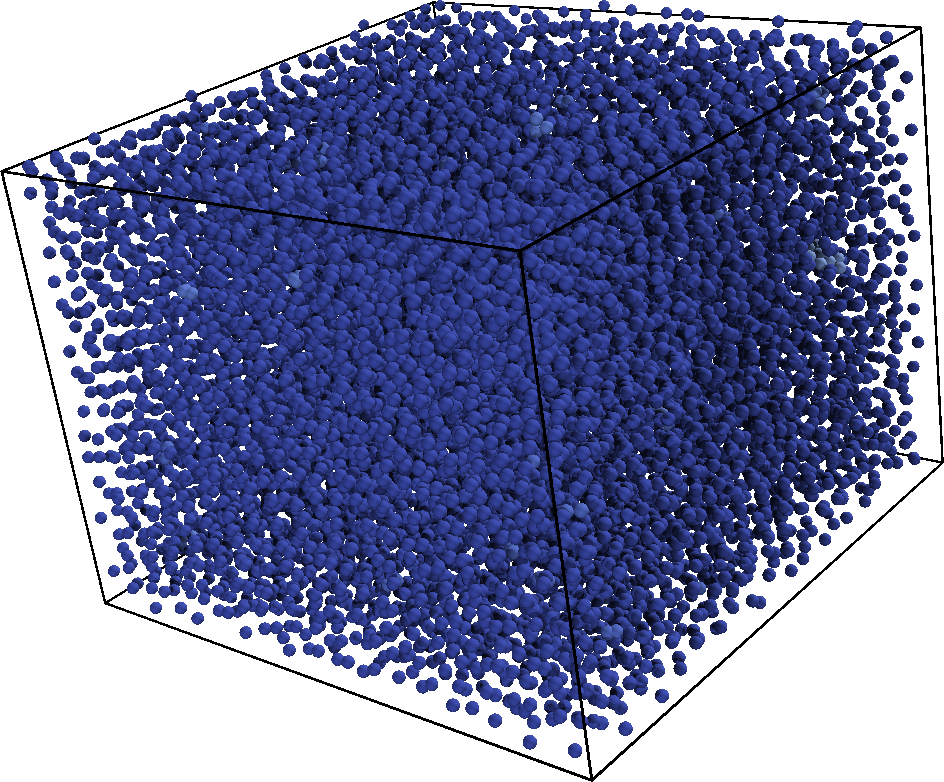
\includegraphics[width=0.3\textwidth]{155C_percolation_1645_p2size_t024.png}};
			\node[below=0.01\textwidth of threeD_5min] (threeD_30min) {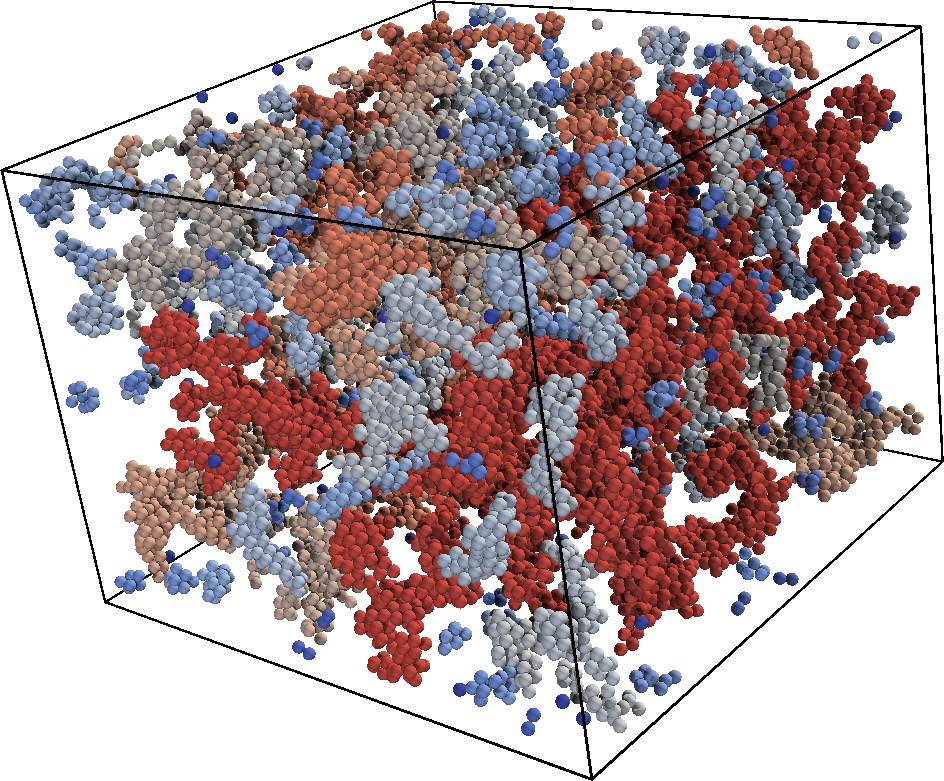
\includegraphics[width=0.3\textwidth]{155C_1715_ageing_p2size_t00.png}};
			\node[right=0.01\textwidth of threeD_30min] (threeD_40min) {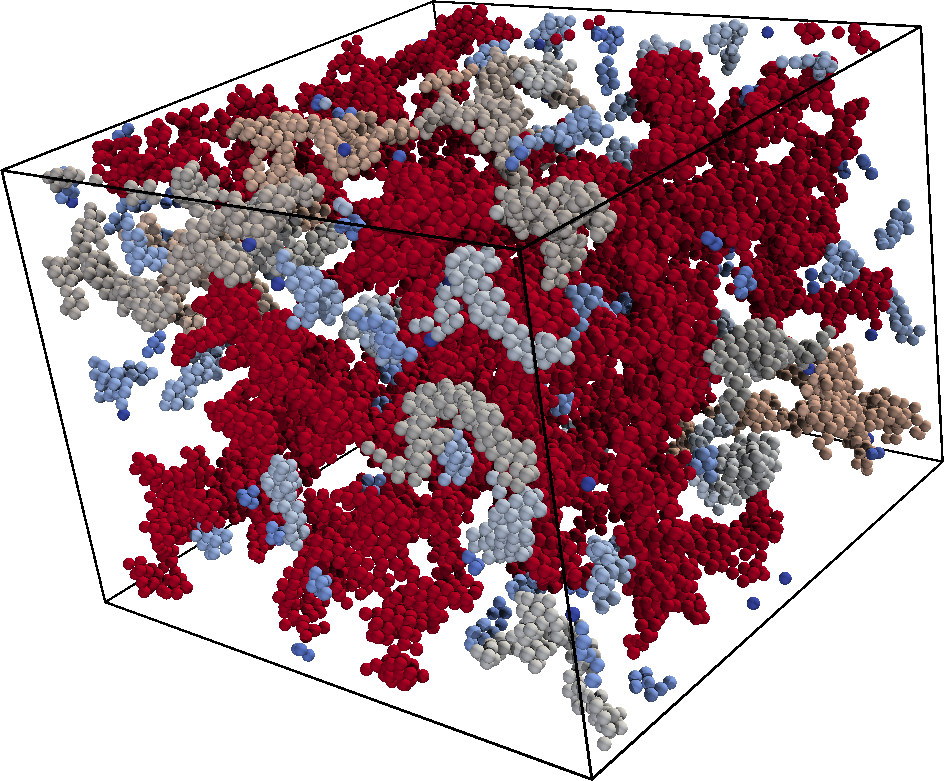
\includegraphics[width=0.3\textwidth]{155C_1715_ageing_p2size_t20.png}};
			\node[right=0.01\textwidth of threeD_40min] (threeD_50min) {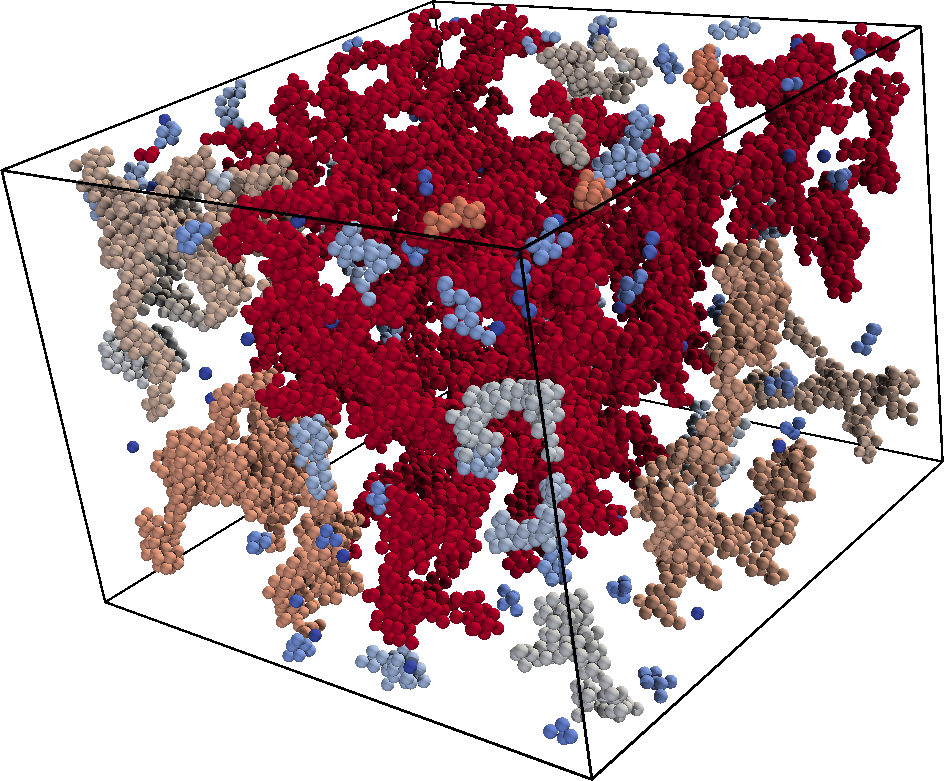
\includegraphics[width=0.3\textwidth]{155C_1715_ageing_p2size_t40.png}};
		\end{scope}
		%\node[right=0.01\textwidth of threeD_10min] (threeD_20min){\includegraphics[width=0.3\textwidth]{3d_draft_20min.jpg}};
		\begin{scope}[lab]
			\node at (threeD_5min.north west) {c};
			\node at (threeD_10min.north west) {d};
			\node at (threeD_20min.north west) {e};
			\node at (threeD_30min.north west) {f};
			\node at (threeD_40min.north west) {g};
			\node at (threeD_50min.north west) {h};
		\end{scope}
		\begin{scope}[above right]
			\node at (threeD_5min.south west) {\SI{5}{\minute}};
			\node at (threeD_10min.south west) {\SI{10}{\minute}};
			\node at (threeD_20min.south west) {\SI{20}{\minute}};
			\node at (threeD_30min.south west) {\SI{30}{\minute}};
			\node at (threeD_40min.south west) {\SI{40}{\minute}};
			\node at (threeD_50min.south west) {\SI{50}{\minute}};
		\end{scope}
	\end{tikzpicture}
	\caption{\textbf{Observing gelation.} \textbf{a} Sketch of our experimental setup. The observation cell contains initially colloids, polymer and no salt. \textbf{b} Phase diagram of our system (the line is a guide for the eye). \textbf{c-h} Early stage of gelation observed experimentally (state point is circled in \textbf{b}). Pictures are computer reconstruction of the experimental coordinates coloured by the number of particles in clusters.}
	\label{fig:methods}
\end{figure*}
\tikzset{external/force remake=false}

\begin{figure}
	\centering
	\begin{tikzpicture}[
		pic3d/.style={inner sep=0}, %
		lab/.style={below left, text height=0.8em, text depth=0.2em, font=\Large\bfseries},%
		every axis/.style={xlabel near ticks, ylabel near ticks, legend cell align=left, legend style={font=\tiny}},%
		]%
		\begin{axis}[%
			width=0.45\textwidth,%
			xlabel={$t/\tau_B$}, xmin=0, xmax=20,%
			ylabel={$R_g/\sigma$}, %ymin=1, %ymax=0.8,%
			]%
			%\node[pic3d, above right] at(axis cs:2.5,1.55) {\includegraphics[width=0.075\textwidth]{N3_0.png}};
			%\node[pic3d, below right] at(axis cs:3,1.45) {\includegraphics[width=0.075\textwidth]{N3_1.png}};
			%\node[pic3d, above left] at(axis cs:20,1.35) {\includegraphics[width=0.075\textwidth]{N3_2.png}};
			\begin{scope}[every node/.style={inner sep=0}]
				\node[circle, ball color=gray] at (axis cs:2.5,1.6) (n3_01){};
				\node[circle, ball color=gray, right=0 of n3_01] (n3_02){};
				\node[circle, ball color=gray, above right= -0.3em and +0.3em of n3_02] (n3_03){};
				\node[circle, ball color=gray] at (axis cs:4,1.4) (n3_11){};
				\node[circle, ball color=gray, below right=-0.3em and 0.3em of n3_11] (n3_12){};
				\node[circle, ball color=gray, above right= +0 and -0 of n3_12] (n3_13){};
				\node[circle, ball color=gray] at (axis cs:18,1.35) (n3_21){};
				\node[circle, ball color=gray, above right=0.2em and -0.3em of n3_21] (n3_22){};
				\node[circle, ball color=gray, right=0 of n3_21] (n3_23){};
			\end{scope}
			\addplot table [x expr=\thisrowno{0}*6, y expr=\thisrowno{1}]{cluster_Rg_dynamics_N3.csv};
			\addplot table [x expr=\thisrowno{0}*6, y expr=\thisrowno{2}]{cluster_Rg_dynamics_N3.csv};
			\addplot table [x expr=\thisrowno{0}*6, y expr=\thisrowno{3}]{cluster_Rg_dynamics_N3.csv};
			\legend{All triplets, Most elongated 20\%, Most compact 20\%};
		\end{axis}
		\begin{semilogxaxis}[%
			at={(0.5\textwidth, 0)},%
			width=0.45\textwidth,%
			xlabel={$t/\tau_B$}, xmin=1, %xmax=200,%
			ylabel={$\phi_\text{eff}$}, ymin=0, ymax=0.8,%
			legend style={legend pos=north west},%
			]%
			\addplot table [x expr=\thisrowno{0}*6-49, y expr=\thisrowno{5}]{201A.csv};
			\addplot table [x expr=(\thisrowno{0}+0.75)*6-45, y expr=\thisrowno{5}]{188B.csv};
			\addplot table [x expr=(\thisrowno{0}+0.75)*6-60, y expr=\thisrowno{5}]{154B.csv};
			\legend{Fluid, Shallow gel, Deep gel};
		\end{semilogxaxis}
		%\node[anchor=south west] at(0.4\textwidth, 0) {\includegraphics[width=0.45\textwidth]{4_EffectiveVolumeFraction_Results.pdf}};
		\begin{semilogxaxis}[%
			at={(0, -0.4\textwidth)},%
			width=0.45\textwidth,%
			xlabel={$t/\tau_B$}, xmin=1, %xmax=160,%
			ylabel={$d_f$}, ymin=1, %ymax=2,%
			legend style={legend pos=south east},%
			no markers,%
			]%
			\addplot table [x expr=\thisrowno{0}/10-49, y expr=\thisrowno{1}]{201A.df};
			%\addplot table [x expr=(\thisrowno{0}+45)/10, y expr=\thisrowno{1}]{155C.df};
			\addplot table [x expr=(\thisrowno{0}+45)/10-45, y expr=\thisrowno{1}]{188B.df};
			\addplot table [x expr=(\thisrowno{0}+45)/10-60, y expr=\thisrowno{1}]{154B.df};
			\legend{Fluid, Shallow gel, Deep gel};
		\end{semilogxaxis}
	\end{tikzpicture}
	\caption{\textbf{Fluid and dilute gel.} \textbf{a} Compaction mechanism of 3-particle-clusters in a fluid. The characteristic time to reach the stable compact cluster is much longer than $\tau_B$. \textbf{b} Effective volume fraction for various percolating and non-percolating samples. Dilute gels reach effective volume fractions comparable to dense phases due to their lack of compactness. \textbf{c-d} Time-evolution of the fractal dimension of the non-percolation clusters below (\textbf{c}) and above (\textbf{d}) the gelation boundary. Insets: typical $d_f$ plots for various times.}
	\label{fig:fluid_dilute}
\end{figure}

%\tikzset{external/force remake}
\begin{figure}
	\centering
	\begin{tikzpicture}[
		pic3d/.style={inner sep=0}, %
		lab/.style={below left, text height=0.8em, text depth=0.2em, font=\Large\bfseries}%
		]%
		\node (im) {%\includegraphics[width=0.4\textwidth]{draft_compaction_dense}
		};
		\node[left=0 of im] {%\includegraphics[width=0.25\textwidth]{draft_nwk_dense_perco}
		};
		\node[right=0 of im] {%\includegraphics[width=0.25\textwidth]{draft_nwk_dense_compact}
		};
		\matrix [below=0of im, inner sep=0.005\textwidth]{%
			\node (arm1) {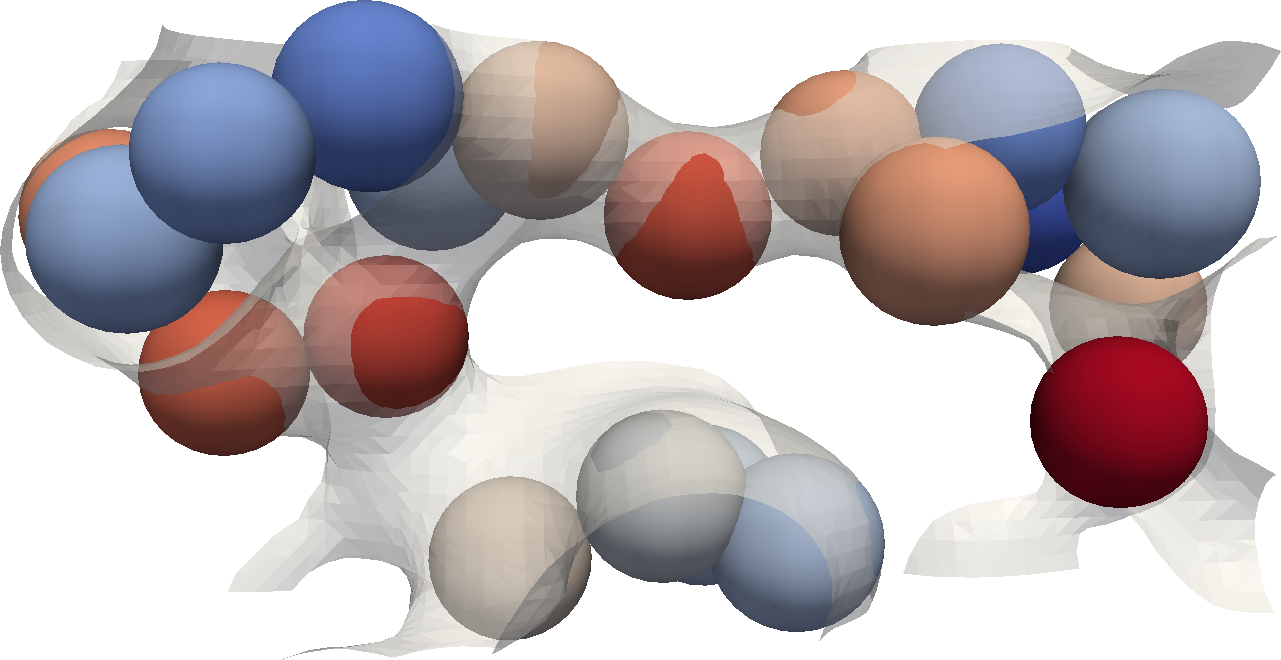
\includegraphics[width=0.3\textwidth]{gaussian_forces_10.png}};&%
			\node (arm2) {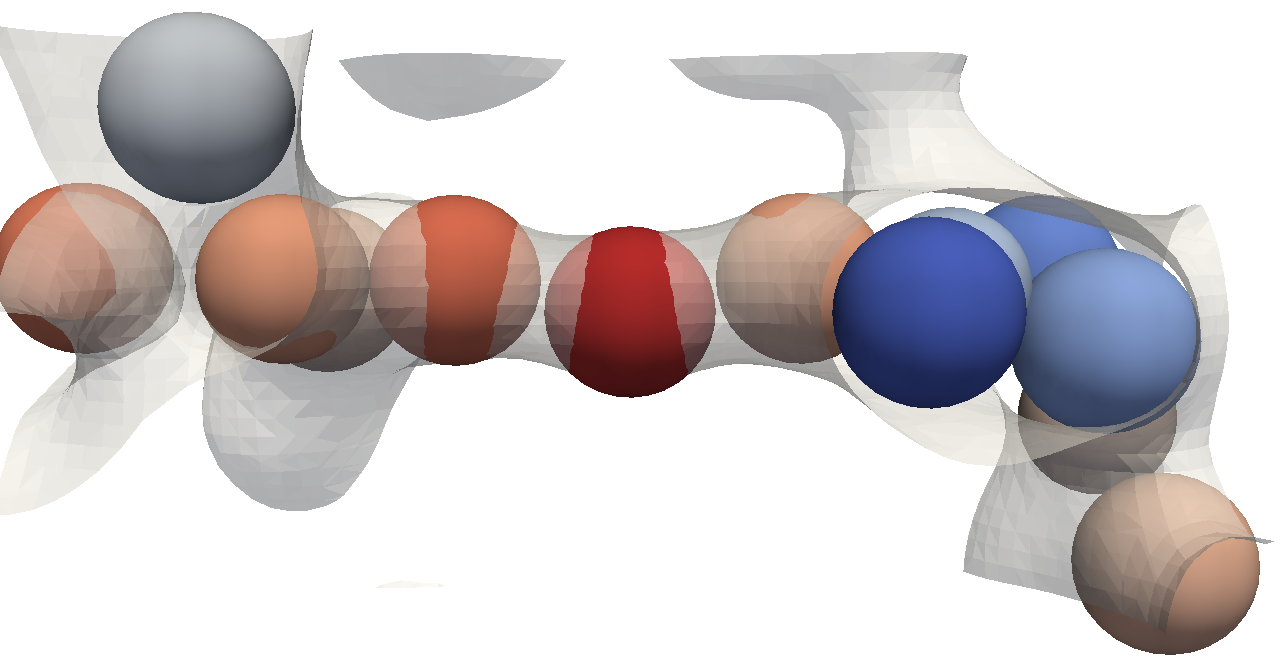
\includegraphics[width=0.3\textwidth]{gaussian_forces_60.png}};&%
			\node (arm3) {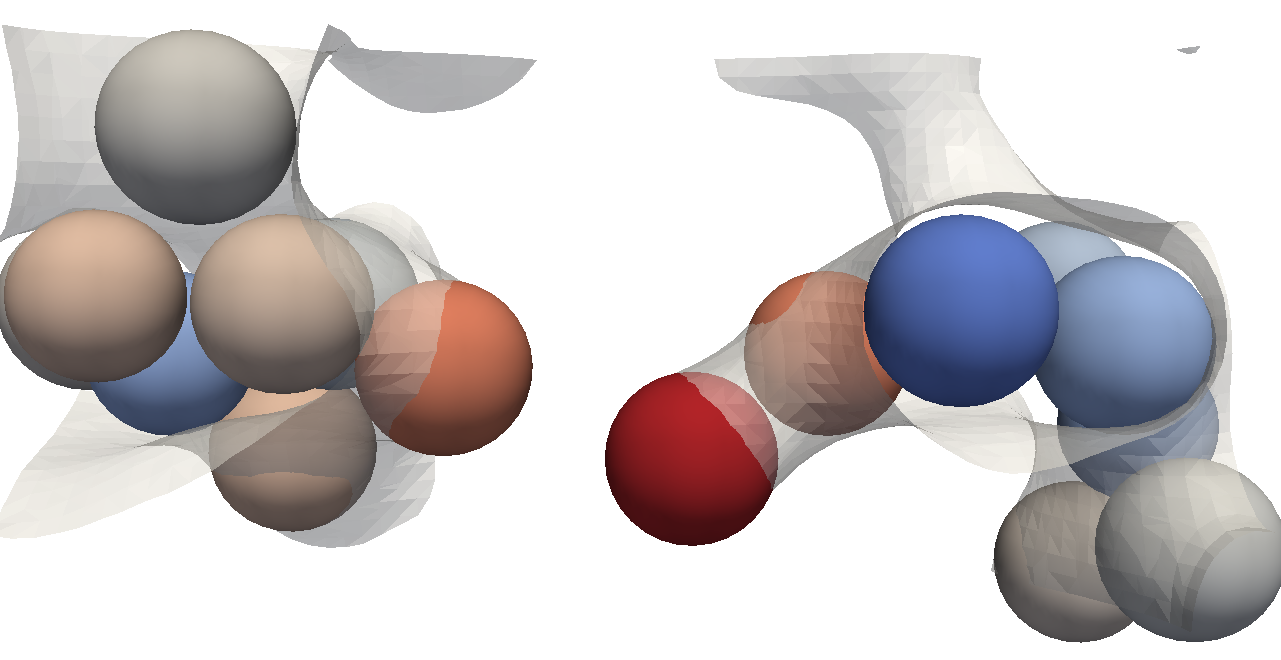
\includegraphics[width=0.3\textwidth]{gaussian_forces_65.png}};\\%
			};
		\node[above right=0 of arm1.south west] {$t=0$};
		\node[above right=0 of arm2.south west] {$t=30\tau_B$};
		\node[above right=0 of arm3.south west] {$t=33\tau_B$};
	\end{tikzpicture}
	\caption{\textbf{Gelation in dense samples.} \textbf{a} Typical time evolution of the largest cluster size and of the mean coordination number. Insets: Confocal images (2D) at percolation and at final stage. \textbf{b-d} Typical arm-breaking event, from relaxed, to stretched, to rupture ($\phi=29~\%$ and $c_p=\SI{0.71}{\gram\per\litre}$). Particles are drawn to scale and colors indicate potential energies from blue (low) to red (high). The smooth surface is a Gaussian coarse-graining of the network pattern. %\textbf{e-f} Typical loop compaction event.  \textbf{b-f} are top views, thus there is no direct role of sedimentation.
	}
	\label{fig:dense}
\end{figure}

\begin{figure}
	%\tikzset{external/force remake}
	\tikzsetnextfilename{hydro}
	\begin{tikzpicture}[lab/.style={below right, text height=0.8em, text depth=0.2em, font=\Large\bfseries}]
		\begin{groupplot}[%
			group style={
				group name=g, group size=2 by 1,
				horizontal sep=4em,
				},
			width=0.5\columnwidth+1em,%
			height=0.5\columnwidth,
			ylabel absolute, every axis y label/.append style={anchor=base, yshift=-1.5em}
			]
			\nextgroupplot[
			xlabel={$t/\tau_B$}, xmin=0, xmax=20,%
			ylabel={$R_g/\sigma$},
			]%
			\addplot table [x expr=\thisrowno{0}*6, y expr=\thisrowno{1}]{cluster_Rg_dynamics_N3.csv} node[pos=0, above right] {all};
			\addplot table [x expr=\thisrowno{0}*6, y expr=\thisrowno{2}]{cluster_Rg_dynamics_N3.csv} node[pos=0, right] {most elongated};
			\addplot table [x expr=\thisrowno{0}*6, y expr=\thisrowno{3}]{cluster_Rg_dynamics_N3.csv} node[pos=0, above right] {least elongated};
			%\legend{All triplets, Most elongated 20\%, Most compact 20\%};
			
		\nextgroupplot[
			width=0.5\columnwidth,
			xlabel={$t/\tau_B$}, xmin=0, xmax=400,
			ymin=0, ymax=1, ylabel={aspect ratio},
			only marks,]
		\addplot table[x expr=\thisrowno{0}*6-19] {172A_1206_percolation.aspect} node[below left] {$\lambda_3/\lambda_1$};
		\addplot table[x expr=\thisrowno{0}*6-19, y index=3] {172A_1206_percolation.aspect} node[above left] {$\lambda_2/\lambda_1$};
	\end{groupplot}
		
	\begin{axis}[
		name=hist,
		anchor=above north west,
		at={(g c1r1.below south west)},
		xlabel={angle (degree)}, xmin=0,xmax=180,%
		ylabel={probability (degree${}^{-2}$)}, ymin=0,
		no markers,%
		width=\columnwidth,
		height=0.6\columnwidth,
		ylabel absolute, every axis y label/.append style={anchor=base, yshift=-1.5em}
		]
			\addplot+[gray!50, fill=gray!50, area legend] file {all.angles} \closedcycle;
			\addplot file {new.angles};
			\addplot+[blue] file {alone.angles};
			\legend{existing, future, isolated};
			
			%sketch future
			\fill[radius=0.6em, red!50] (axis cs:20,0.02) circle[] +(0,1.2em) circle[] ++(1.2em,0) circle[] +(-120:1.2em) circle[];
			\draw[ultra thick] (axis cs:20,0.02) -- ++(1.2em,0) -- +(-120:1.2em);
			\draw[thick, dotted] (axis cs:20,0.02) +(1.2em,0) -- +(0,1.2em);
			
			%sketch alone
			\fill[radius=0.6em, blue!50] (axis cs:90,0.04) circle[] +(-1.2em,0) circle[] +(-120:1.2em) circle[] +(30:1.5em) circle[];
			\draw[ultra thick] (axis cs:90,0.04) -- +(-1.2em,0) (axis cs:90,0.04)-- +(-120:1.2em);
			\draw[thick, dotted] (axis cs:90,0.04) -- +(30:1.5em);
		\end{axis}
			
		\node[lab] at (g c1r1.outer north west) {a};
		\node[lab] at (g c2r1.outer north west) {b};
		\node[lab] at (hist.outer north west) {c};
	\end{tikzpicture}
	\caption{\textbf{Hydrodynamics} \textbf{a} Evolution of triplet radii of gyration in a non percolating sample ($\phi=4~\%$, $c_p=\SI{1}{\gram\per\litre}$). The characteristic time to reach the stable compact cluster is much longer than the Brownian time. \textbf{b} Evolution of the aspect ratios of clusters of 4 particles and more in a percolating sample ($\phi=8~\%$, $c_p=\SI{1.5}{\gram\per\litre}$) \textbf{c} Bond angle distribution relative to existing bonds (gray), to a future bond (red) or to a future bond involving an isolated particle (blue). Future bonds are shifted to smaller angles, whereas gas adsorption takes place from larger angles. Insets sketch both cases, with present bonds drawn thick and future bonds drawn dotted.}
	\label{fig:hydro}
\end{figure}
%\tikzset{external/force remake=false}

\begin{figure*}
	\tikzset{external/force remake}
	\tikzsetnextfilename{cell_vs_cap}
	\begin{tikzpicture}[
		pic3d/.style={inner sep=0}, %
		lab/.style={below right, text height=0.8em, text depth=0.2em, font=\Large\bfseries},%
		]%
		%box
		\draw[every node/.style={draw, inner sep=0, minimum width=0.01\textwidth, minimum height=0.12\textwidth, anchor=south west}] 
			node (Rrightwall) at (0, 0) {}
			node (Rleftwall) at (0.2\textwidth, 0) {}
			[every node/.append style={minimum height=0.06\textwidth}]
			node (Crightwall) at (0, 0.13\textwidth) {}
			node (Cleftwall) at (Crightwall.south -| Rleftwall.west) {}
			(Crightwall.north west) +(0,0.005\textwidth) rectangle (Cleftwall.north east);
			
	
		%filtre
		\foreach \x / \y in {0/0.23, 0.27/0.48, 0.52/0.73, 0.77/1}
			\fill[gray] ($(Rrightwall.north west)!\x!(Rleftwall.north east)$) rectangle ($(Crightwall.south west)!\y!(Cleftwall.south east)$);
		
		
		%laser
		\node[fill, green, semitransparent, isosceles triangle, anchor=apex, shape border rotate=-90, minimum width=0.08\textwidth, inner sep=0,  isosceles triangle apex angle=75] at ($(Crightwall.north east)!0.4!(Cleftwall.south west)$) (laser) {};
		
		%lens
		\filldraw[lightgray] (laser.right corner) arc[start angle=180,delta angle=180,x radius=0.04\textwidth, y radius=0.01\textwidth] --cycle;
		%colloids
		\begin{scope}[radius=0.008\textwidth, ball color=red!80]
			\shade(0.08\textwidth, 0.175\textwidth) circle;
			\shade(0.11\textwidth, 0.16\textwidth) circle;
			\shade(0.05\textwidth, 0.15\textwidth) circle;
			\shade(0.03\textwidth, 0.18\textwidth) circle;
			\shade(0.14\textwidth, 0.14\textwidth) circle;
			\shade(0.16\textwidth, 0.165\textwidth) circle;
		\end{scope}
		
		%polymers
		\foreach \x / \y in {0.06/0.1745, 0.17/0.1345, 0.172/0.14, 0.145/0.16, 0.19/0.18, 0.09/0.14, 0.03/0.15} 
			\draw[%
			gray, decoration={coil, segment length=0.0025\textwidth, amplitude=0.0025\textwidth},
			] (\x\textwidth, \y\textwidth)
			decorate{++(-0.0025\textwidth,-0.0025\textwidth) -- ++(0.0045\textwidth,0.0045\textwidth) -- ++(0,-0.0045\textwidth) -- ++(-0.005\textwidth,+0.005\textwidth) };
		
		
		%salt
		\begin{axis}[
			at={($(Rrightwall.south east)+(0.75,0.75)$)},
			width=0.19\textwidth-2*0.75,
			height=0.115\textwidth,
			axis lines=none,
			scale only axis,
			xmin=-1, xmax=1,ymin=0,ymax=1,
			]
			\addplot [blue, only marks, mark=*, samples=1000, mark size=0.75]
    {rand^2};
		\end{axis}
		
		%arrows
		\foreach \x in {0.25,0.5,0.75}
			\draw[blue!20,->, line width=0.005\textwidth] ++($(Rrightwall.south west)!\x!(Rleftwall.south east)$) +(0, 0.08\textwidth) -- +(0, 0.11\textwidth);
		
		
		%labels
		\begin{scope}[right, font=\footnotesize]
			\node[above right=0 of Rleftwall.south east] (Reservoir) {Reservoir};
			\node[anchor=north west] at (laser.lower side-|Reservoir.west) {Objective lens};
			\node at (Cleftwall-|Reservoir.west) (oc) {Observation cell};
			\node[anchor=base west] at (Rleftwall.north-|Reservoir.west){Filter};
			\node[above right,blue] at (Rleftwall.east-|Reservoir.west) {Salt diffusion};
			%\node[above right] at (0.21\textwidth, 0) {Reservoir};
		\end{scope}
			
		\node[inner sep=0pt,thick,fit=(Rrightwall) (oc) (laser)
		] (cellsketch) {};
		\node[lab, below right=0, inner sep=0] at (cellsketch.north west) {a};
		
		%%%%Capillary vs Reservoir Cell%%%
		\node[inner sep=0, below right=0 and 1em of cellsketch.north east] (ResSnapshot) {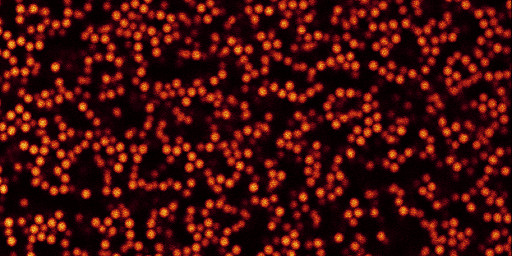
\includegraphics[width=0.2\textwidth]{Res362A_scan2Snapshot1.jpg}};
		\node[inner sep=0, above right=0 and 1em of cellsketch.south east] (CapSnapshot) {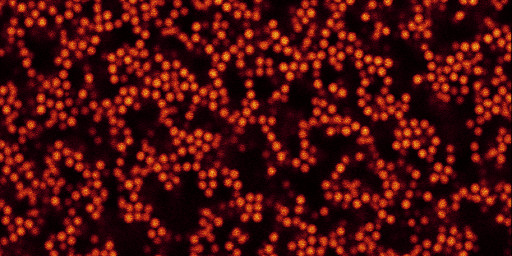
\includegraphics[width=0.2\textwidth]{Cap362_Snapshot1.jpg}};
		\node[lab,white] at (ResSnapshot.north west) {b};
		\node[lab,white] at (CapSnapshot.north west) {c};
		
		%%%%Phase diagram%%%%
		
		\begin{axis}[%
			at={($(cellsketch.north west)+(\textwidth,0)$)}, anchor=outer north east,%
			name={phasediag},%
			width=0.425\textwidth, height=0.3\textwidth,%
			xmin=0, xmax=40, xlabel={$\phi$}, x unit={\%},
			ymin=0.08, ymax=3.5, ylabel={$c_p$}, y unit={\si{\gram\per\litre}},%
			%ytick={0.1,0.2,0.3,0.4,0.5,0.6,0.7,0.8,0.9,1,2}, yticklabels={0.1,0.2,,,0.5,,,,,1,2},%
			legend pos=north east,%
			legend style={font=\footnotesize},%
			only marks,%
			]%
			\addplot[sharp plot, no marks] table [x expr=100*\thisrowno{0}, y index=1] {gasliquid_sg.phd};
			%\addplot[sharp plot, no marks, dashed] table [x expr=100*\thisrowno{0}, y index=1] {gasliquid_bg.phd};
			%\addplot[sharp plot, no marks, dotted] table [x expr=100*\thisrowno{0}, y index=1] {fluidsolid_f.phd};
			%\addplot+[forget plot] table [x index=1,y index=2] {phase_diag_capillary.csv};
			\addplot table [x index=1,y index=2] {phase_diag_gel.csv};
			\addplot table [x index=1,y index=2] {phase_diag_fluid.csv};
			\addplot table [x index=1,y index=2] {phase_diag_clusters.csv};
			\legend{spinodal, gel, fluid, clusters};
			\node[circle, draw, gray] at (axis cs:7.4, 0.98) (155C) {};
			\node[draw, gray] at (axis cs:25.7, 1.43) (Cap1) {};
		\end{axis}
		\node[lab] at (phasediag.outer north west) {d};
		
		%scale bar
		\draw[ultra thick] node[anchor=south east, inner xsep=0] (sb) at (CapSnapshot.south east |- phasediag.outer south)  {\SI{50}{\micro\metre}} (sb.north east) -- +(-0.069\textwidth,0);
	\end{tikzpicture}
	\caption{\textbf{Reservoir cell} \textbf{a} Sketch of our experimental setup. The observation cell contains initially colloids, polymer and no salt. \textbf{b} Confocal picture of a gel formed in situ ($\phi=25.5~\%$, $c_p=\SI{1.4}{\gram\per\litre}$), \SI{1}{\hour} after gelation. \textbf{c} Confocal picture of a gel at the same state point formed ex situ, \SI{1}{\hour} after shear melting. \textbf{d} Phase diagram obtained in reservoir cell. Spinodal line is obtained from free volume theory.}
	\label{fig:cell_vs_cap}
\end{figure*}


\begin{figure}
	\tikzset{external/force remake}
	\tikzsetnextfilename{wholeprocess}
	\begin{tikzpicture}[
		lab/.style={below right, text height=0.8em, text depth=0.2em, font=\Large\bfseries},%
		]
	\pgfplotscreateplotcyclelist{earthy}{%
	black,
	red!40!black,
	red!60!black,
	red!80!black,
	red,
	red!80!yellow,
	red!60!yellow,
	red!40!yellow,
	}
	\begin{groupplot}[
	group style={
			group name=g, group size=2 by 1,
			horizontal sep=4em,
			},
		width=0.5\columnwidth+1em,%
		height=10\baselineskip,%
		ylabel absolute, every axis y label/.append style={anchor=base, yshift=-1.5em}
		]
%		\nextgroupplot[
%			xlabel={time (min)}, xmin=0,
%			ymin=0, ymax=1, ylabel={aspect ratio},
%			only marks,]
%		\addplot table {155C_percolation_1645.aspect} node[below left] {$\lambda_3/\lambda_1$};
%		\addplot table[y index=3] {155C_percolation_1645.aspect} node[above left] {$\lambda_2/\lambda_1$};
		\nextgroupplot[
			xlabel=$q^2\sigma^2$, xmin=0,
			ylabel=$A\tau_B/q^2\sigma^2$, ymin=0, ymax=0.2, ytick={0,0.1,0.2},
			]
		\addplot[only marks] table[x expr=\thisrowno{0}^2, y expr=\thisrowno{1}/\thisrowno{0}^2] {155C.growth};
		\addplot[no marks, red, domain=1.6:7] {1.5*(1-0.115*x)/(1+3.62*x)}; 
		
		\nextgroupplot[
			xmode=log, ymode=log,
			xlabel={$(t-t_0)/\tau_B$}, xmin=1,
			ylabel=$\langle q\rangle\sigma$, ymin=0.6,
			ytick={0.6,0.8,1,1.2,1.6,2}, yticklabels={0.6, 0.8,1,1.2,1.6, 2},
			]
		\addplot[only marks] table[x expr=6*(\thisrowno{0}-5)]{155C.qmax};
		\addplot+[red, no marks, domain=20:200] {4*x^(-1/3)} node[midway, below left]{$-1/3$};
	\end{groupplot}

	\begin{axis}[name=Sq,
		anchor=below south west,
		at={(g c1r1.above north west)},
		xmin=0, xmax=13, ymin=0,
		xlabel=$q\sigma$, ylabel=$S(q)$,
		ylabel absolute, every axis y label/.append style={anchor=base, yshift=-1.5em},
		scale only axis,
		width=\columnwidth-3.5em,
		height=6\baselineskip,
		no marks, cycle list name=earthy]
		\foreach \ii in {1,2,...,7}
			\addplot table[y index=\ii] {155C_every150s.Sqs};
		\draw[<-] (axis cs:3.1,3.3) -- +(45:1em) node[right]{Wigner};
		\draw[<-,red!80!black] (axis cs:6.5,1.9) -- +(45:1em) node[right]{Hard sphere};
		\draw[<-,red!60!yellow] (axis cs:0.8,7.5) -- +(0:1em) node[right]{Gelation};
	\end{axis}

	
	\matrix[
		matrix of nodes, inner sep=0, column sep=0.01\textwidth, row sep=0.5em,
		matrix anchor=south west,
		%at={($(g c1r1.outer north west)$)},
		at={($(Sq.outer north west)+(0,1em)$)},
		] (m){
		\SI{0}{\minute} & \SI{5}{\minute} \\
		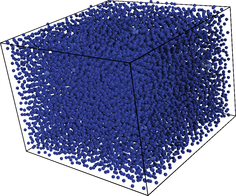
\includegraphics[width=0.48\columnwidth]{155C_percolation_1645_p2size_t024s.png}&
		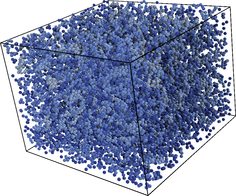
\includegraphics[width=0.48\columnwidth]{155C_percolation_1645_p2size_t044s.png}\\
		\SI{15}{\minute} & \SI{25}{\minute}\\
		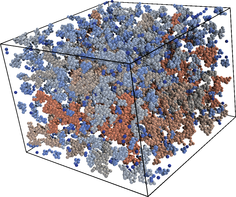
\includegraphics[width=0.48\columnwidth]{155C_percolation_1645_p2size_t084s.png} &
		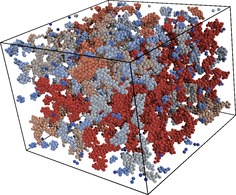
\includegraphics[width=0.48\columnwidth]{155C_1715_ageing_p2size_t00s.png}\\
		 \SI{35}{\minute} & \SI{45}{\minute}\\
		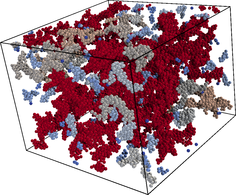
\includegraphics[width=0.48\columnwidth]{155C_1715_ageing_p2size_t20s.png}&
		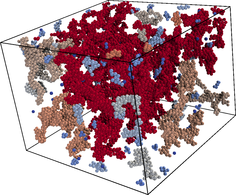
\includegraphics[width=0.48\columnwidth]{155C_1715_ageing_p2size_t40s.png}\\
		};
	\node[lab] at (m.north west) {a};
	\node[lab] at (Sq.outer north west) {b};
	\node[lab] at (g c1r1.outer north west) {c};
	\node[lab] at (g c2r1.outer north west) {d};
	\end{tikzpicture}
\caption{\textbf{Gelation observed in-situ} in a typical sample ($\phi=7.5~\%$, $c_p=\SI{1}{\gram\per\litre}$). Origin of time is the last frame before melting of Wigner crystal. \textbf{a} Reconstruction of experimental coordinates coloured by the number of particles in clusters. \textbf{b} Structure factor evolution (a curve every \SI{150}{\second}). \textbf{c} Cahn plot of the initial growth rate $A(q)$. The line is a fit by Eq. XXX with $\xi=0.11\sigma$ and $\xi_{ve}=3.6\sigma$. \textbf{d} Growth of the characteristic wave number.}
\label{fig:wholeprocess}
\end{figure}



\end{document}